\documentclass{article}
\usepackage{listings}
\usepackage{color}
\usepackage{float}
\usepackage{graphicx}

\definecolor{dkgreen}{rgb}{0,0.6,0}
\definecolor{gray}{rgb}{0.5,0.5,0.5}
\definecolor{mauve}{rgb}{0.58,0,0.82}

\lstset{
	frame=single,
	language=C,
	belowskip=3mm,
	showstringspaces=false,
	columns=flexible,
	captionpos=b,
	basicstyle={\small\ttfamily},
	numbers=left,
	numbersep=5pt,
	%numbers=none,
	numberstyle=\tiny\color{gray},
	keywordstyle=\color{blue},
	commentstyle=\color{dkgreen},
	stringstyle=\color{mauve},
	breaklines=true,
	breakatwhitespace=true,
	tabsize=4
}

\input kvmacros
\sloppy
\begin{document}

\title{Project 4: File System}
\author{\textit{Yesheng Ma}}
\date{\today}
{\bf\small CS353: Linux Kernel}\hfill{\bf\small 2017 Spring}
{\let\newpage\relax\maketitle}
\maketitle


\begin{abstract}
In this project, we will mount a romfs image to our virtual machine and do some modifications to the romfs Linux kernel model to accomplish several tasks.
\end{abstract}

\section{Introduction to romfs}
\emph{Romfs} is a space-efficient, small, read-only filesystem originally for Linux and used by some Linux based projects. In this project, our main goals are:
\begin{itemize}
\item Mount a romfs to your system.
\item Change romfs code to hide a file/directory.
\item Change the code to read an encrypted romfs file.
\item Change the execution bit and modify display format of a file.
\end{itemize}

\section{Basic romfs Build and Mount}
The source code of romfs project is maintained at \texttt{romfs.sourceforge.net}. We can generate a romfs image using the \texttt{genromfs} tool. You can build \texttt{georomfs} from source or if you are using Debian-based Linux, you can directly install it from package manager by \texttt{apt install genromfs}.

We can create a romfs image by executing \texttt{genromfs -f fs.img -d dir} where \texttt{dir} is the directory to be transformed. To mount the romfs, execute \texttt{mount -o loop fs.img mnt}, where \texttt{mnt} is the directory to be mounted and maybe superuser privilege is needed.

\begin{figure}[H]
\centering
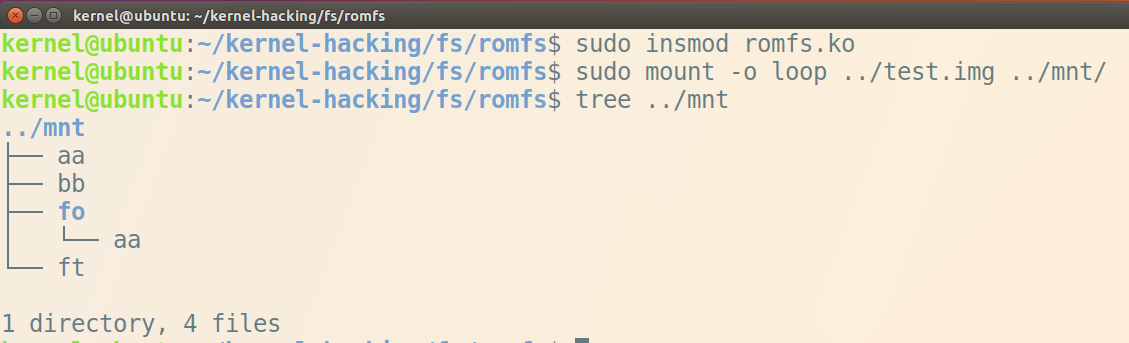
\includegraphics[width=10cm]{basic.png}
\caption{Romfs mount}
\end{figure}

\section{Hide a romfs File}
To hide a file in a romfs, we need to do something in the file loop-up routine. When we see a file matching the name to be hided, we need to explicit set the return inode value to \verb|NULL| so that other routines calling \verb|romfs_lookup| will regard this file as if it does not exist.

\begin{lstlisting}[caption=Code for file hiding]
// in romfs_readdir
if(hide_file_name!=NULL)
    ret =romfs_dev_strcmp(i->i_sb, offset+ROMFH_SIZE, hide_file_name,j);
else
	ret = 0;

// in romfs_lookup
if (hide_file_name != NULL && strcmp(name,hide_file_name == 0))
    inode = NULL;
\end{lstlisting}

\begin{figure}[H]
\centering
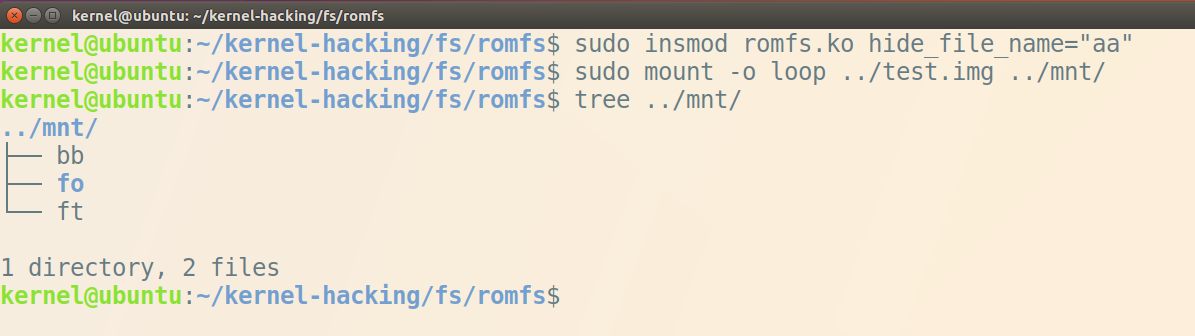
\includegraphics[width=10cm]{hide.png}
\caption{File hiding}
\end{figure}


\section{Encrypt a romfs File}
Since in previous projects, we are all ready quite familiar with how Linux handles file context display. We know that to display the content of a file, we are actually write to a buffer at a particular address offset. We first verify whether we want to encrypt a file and then if the file needs encryption, we write \verb|*| to the respective buffer.

\begin{lstlisting}[caption=Code for encryption]
// in romfs_readpage
int encrypt=0;
if (encry_file_name != NULL)
	if (strcmp(fsname,encry_file_name) == 0)
		encrypt=1;
...
if (encrypt == 1) {
	memset(buf,'*',fillsize-1);
	*((char *)buf + fillsize-1) = '\n';	
}
\end{lstlisting}

\begin{figure}[H]
\centering
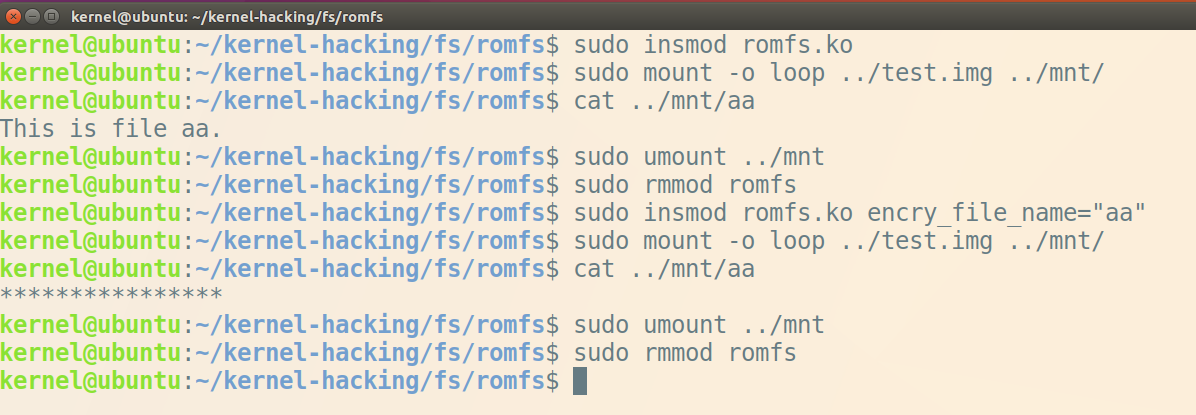
\includegraphics[width=10cm]{encry.png}
\caption{File encryption}
\end{figure}

\section{Change Execution Bit}
To change the execution bit of a file, when the inode is indexed, we need to change the \verb|mode| in the inode struct. If the change execution bit option is enabled and the file name matches the target file name, we simply do a mode maks to enable the execution bit.

\begin{lstlisting}[caption=Code for encryption]
// in romfs_iget
if (addex_file_name != NULL && strcmp(fsname,addex_file_name) == 0)
	mode |= S_IXUGO;
\end{lstlisting}

\begin{figure}[H]
\centering
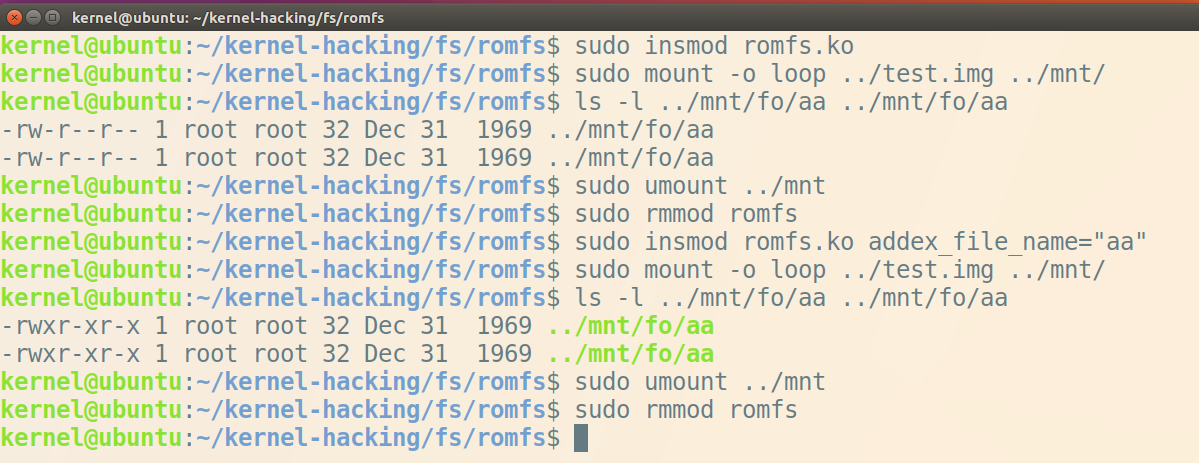
\includegraphics[width=10cm]{exec.png}
\caption{File execution bit}
\end{figure}


\section{Conclusion}
Virtual file system(VFS) is an important abstraction in the Linux kernel. In this project, we learned the romfs, one of the many file systems that support VFS API. This may benefit us when we learn other file systems later.

\section*{Acknowledgement}
Thanks Prof. Chen for guidance on Linux kernel and TAs for their hard work.
\end{document}
